\chapter{Постановка задачи и описание исходных данных} \label{ch1}

% не рекомендуется использовать отдельную section <<введение>> после лета 2020 года
%\section{Введение. Сложносоставное название первого параграфа первой главы для~демонстрации переноса слов в содержании} \label{ch1:intro}


\section{Постановка задачи} \label{ch1:sec1}
Задача заключается в модификации и улучшении механизма обработки изображений реализованного в пакете \textbf{ProStack} \cite{prostack}.

В работе будут подробно описаны модификации, улучшения, и новые методы встроенные в пакет. 


\section{Описание исходных данных} \label{ch1:sec2} 


 Исходные данные представляют собой трехмерные двухканальные изображения полученные с помощью конфокального микроскопа(тут хочется написать про автора этих изображений).
 
Современные конфокальные микроскопы обычно имеют несколько
фотоприемных каналов, благодаря которым можно получить изображения
одновременно в нескольких спектральных областях, т.е. использовать
несколько флуорохромов. 
\begin{figure}[H]
	\centering
	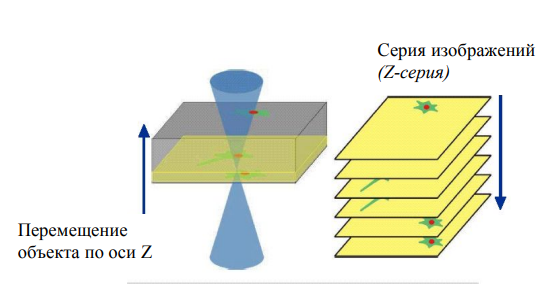
\includegraphics[width=7cm, height=7cm]{z_imgs}
	\caption{Получение серии оптических срезов(Z-серия).}
	\label{z_imgs}
\end{figure}

\begin{figure}[H]
	\centering
	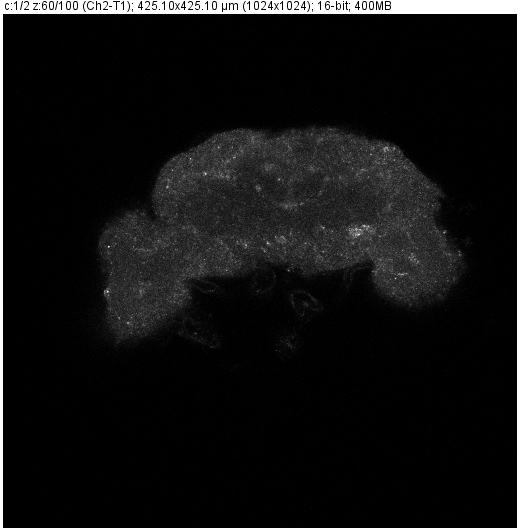
\includegraphics[width=8cm, height=10cm]{in_example}
	\caption{Пример трехмерного двухканального изображения мозга плодовой мушки.}
	\label{in_example}
\end{figure}



\section{Сложность задачи} \label{ch1:sec3}
Существует некоторая проблема в решении поставленной задачи. В исходных изображениях наблюдается паразитное свечение из одного канала микроскопа в другом, что вредит выделению частиц. Данное явление называется автофлуоресценцией. Существует несколько методов решения этой проблемы, которые позволяют уменьшить этот эффект, однако конкретный метод и параметры надо тестировать с конкретными изображениями. Также может понадобиться проводить предобработку и модифицировать последующие шаги всей процедуры. 

\section{Существующие методы решений} \label{ch1:sec4}
\begin{figure}[H]
	\centering
	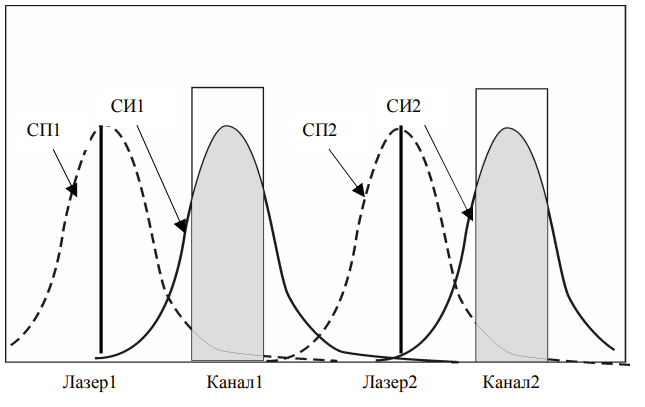
\includegraphics[width=8cm, height=6cm]{c1_c2_norm}
	\caption{Перекрытие спектров полностью отсутствует. СП –
		спектры поглощения, СИ – спектры испускания флуорохромов 1 и 2.}
	\label{c1_c2_norm}
\end{figure}

\begin{figure}[H]
	\centering
	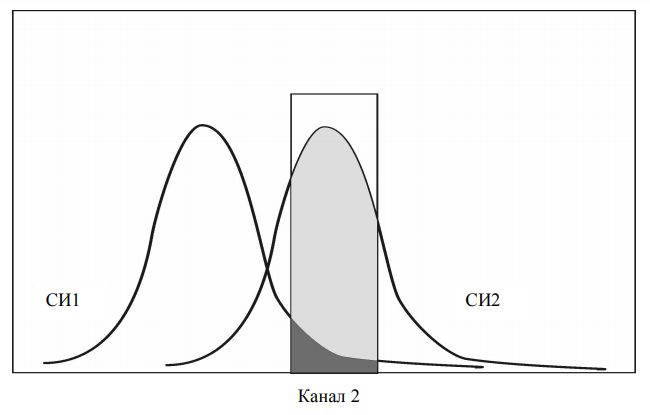
\includegraphics[width=8cm, height=6cm]{c1_c2_bad}
	\caption{Слабое перекрытие спектров. Обозначения те же.}
	\label{c1_c2_bad}
\end{figure}

\begin{figure}[H]
	\centering
	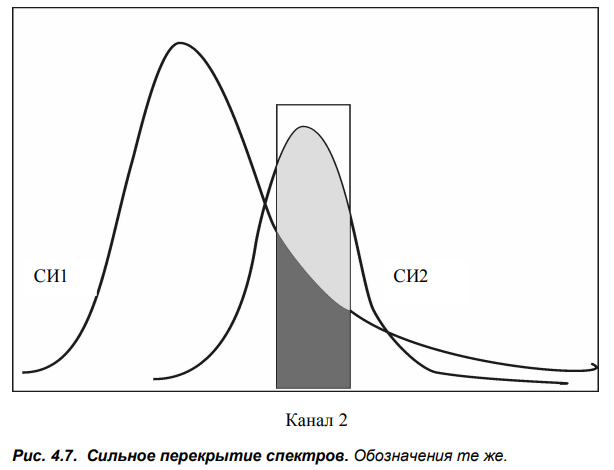
\includegraphics[width=8cm, height=6cm]{c1_c2_baddd}
	\caption{Сильное перекрытие спектров. Обозначения те же}
	\label{c1_c2_baddd}
\end{figure}


Существуют следующие возможные случаи взаимодействия сигналов от двух
флуорохромов. Наилучший вариант показан на Рис.\ref{c1_c2_norm} Перекрытия
спектров нет.



На Рис. \ref{c1_c2_bad} представлен вариант со слабым перекрытием спектров. Часть
спектра испускания первого флуорохрома попадает во второй фотоприемный
канал. Для это случая нужна небольшая предобработка. Уменьшить перекрытие можно путём уменьшения мощности первого лазера. Чтобы  яркость изображения не падала, нужно усилить первый канал, а также сдвинуть полосу приема второго канала вправо.

 В последнем случаем - когда перекрытие сильное(Рис. \ref{c1_c2_baddd}) необходимо применять последовательное сканирование. То есть сначала включить лазер и фотоприемник для первого канала, затем отключить и потоврить для второго канала (режим Multitrack на LSM).
 
Также существует программный способ уменьшения перекрытия
спектров. Он основан на различных математических алгоритмах, учитывающих
информацию о спектрах применяемых красителей, применяющих методы
линейной алгебры, адаптивном или ручном разделении изображений по
приемным каналам. Именно такой способ будет рассмотрен в данной работе.

Наиболее эффективным способом избежания перекрытия спектров является последовательное сканирование, однако у этого подхода есть несколько ограничений.Он требует использования специализированного оборудования и запатентованного программного обеспечения, что является ограничивающим фактором в его широком использовании. Также, например, получения изображений для каждого фотоприемного канала значительно увеличивает время получения изображений и объем данных.




%\FloatBarrier % заставить рисунки и другие подвижные (float) элементы остановиться

%% Вспомогательные команды - Additional commands
%
%\newpage % принудительное начало с новой страницы, использовать только в конце раздела
%\clearpage % осуществляется пакетом <<placeins>> в пределах секций
%\newpage\leavevmode\thispagestyle{empty}\newpage % 100 % начало новой страницы